Se detallan los diferentes diagramas de clases de los restantes tres archivos de la carpeta entrenarmodelos, estos archivos contienen la implementación de los diversos modelos propuestos:

\begin{itemize}

\item cnn\_tres.py: Crea los modelos de redes convolucionales propuestos con una arquitectura base de tres capas, para más detalles ver la figura \ref{fig:uml9}.

\begin{figure}[h!]
	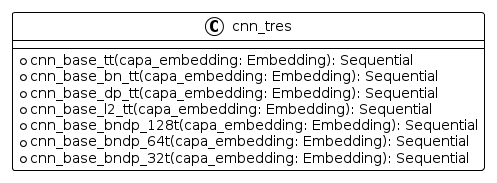
\includegraphics[width=0.65\textwidth]{capitulo5/figuras/fig9.png}
	\caption{Diagrama de clase del archivo cnn\_tres
		\\\textit{Fuente: Elaboración Propia}}
	\label{fig:uml9}
\end{figure}

\item cnn\_four.py: Crea los modelos de redes convolucionales propuestos con una arquitectura base de cuatro capas, para más detalles ver la figura \ref{fig:uml10}.

\begin{figure}[h!]
	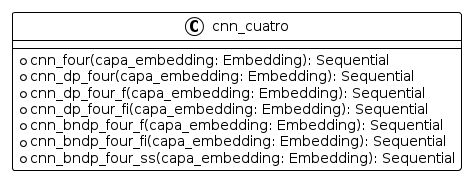
\includegraphics[width=0.6\textwidth]{capitulo5/figuras/fig10.png}
	\caption{Diagrama de clase del archivo cnn\_cuatro
		\\\textit{Fuente: Elaboración Propia}}
	\label{fig:uml10}
\end{figure}

\item cnn\_dos.py: Crea los modelos de redes convolucionales propuestos con una arquitectura base de dos capas, para más detalles ver la figura \ref{fig:uml11}.

\begin{figure}[h!]
	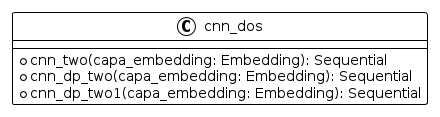
\includegraphics[width=0.5\textwidth]{capitulo5/figuras/fig11.png}
	\caption{Diagrama de clase del archivo cnn\_dos
		\\\textit{Fuente: Elaboración Propia}}
	\label{fig:uml11}
\end{figure}

\end{itemize}

Para cada modelo propuesto, se guarda una copia en cualquier época durante el entrenamiento en la que la pérdida del conjunto de validación disminuya. Además, para mayor comodidad, se almacena todo el historial de entrenamiento de cada modelo, permitiendo visualizar su avance y realizar comparaciones con otros modelos.

